\documentclass{article}

% set font encoding for PDFLaTeX or XeLaTeX
\usepackage{ifxetex}
\ifxetex
  \usepackage{fontspec}
\else
  \usepackage[T1]{fontenc}
  \usepackage[utf8]{inputenc}
  \usepackage{lmodern}
\fi
\usepackage{graphicx}

% used in maketitle
\title{Actividad 3}
\author{Jesús Adrián Zatarain Alvarado}
\date{14 de febrero del 2018}
% Enable SageTeX to run SageMath code right inside this LaTeX file.
% documentation: http://mirrors.ctan.org/macros/latex/contrib/sagetex/sagetexpackage.pdf
% \usepackage{sagetex}

\begin{document}
\maketitle

\section{Introducción}

En la actividad se tienen que observar los fenómenos naturales que se hacen más notables cuando aumentas o decreces en la altura en la que te encuentras. Conforme estás más arriba, ingresas a las distintas etapas que conforman la atmófera terrestre. Ciertos fenómenos son más o menos acentuados en las distintas capas. Para ello se graficarán en un plano bidimensional con el propósito de observarlos y tener una idea más general de su distribución respecto a la altura.
En la actividad se pide obtener los datos de los fenómenos meteorológicos de junio y diciembre de una localidad cualquiera del planeta.

\section{Fundamentos}

La atmósfera consiste en 4 capas. Es en donde ocurren los distintos fenómenos y son más o menos acentuados respecto a qué etapa se encuentran de la atmósfera. a continuación se enumeran las distintas capas que tiene la atmófera y así como su pequeña descripción, acentuando su importancia.

\itemize

\item Troposfera: Es la parte de la atmófera terrestre que está en contacto con la superficie de la Tierra. Tiene alrededor de 17 km de espesor en el ecuador terrestre y solo 7 km en los polos, y en ella ocurren todos los fenómenos meteorológicos que influyen en los seres vivos, como los vientos, la lluvia y la nieve. Además, concentra la mayor parte del oxígeno y del vapor de agua. En particular esta capa actúa como un regulador térmico del planeta; sin ella, las diferencias térmicas entre el día y la noche serían tan grandes que no podríamos sobrevivir. Es de vital importancia para los seres vivos. La troposfera es la capa más delgada del conjunto de las capas de la atmósfera.

\item Estratósfera: Está situada entre la troposfera y la mesósfera. La altura a la que comienza es variable: En las regiones polares a menor altura, entre 6 y 9 kilómetros o más; y en las regiones ecuatoriales entre 16 y 20 kilómetros. Se extiende hasta los 50 km de altura aproximadamente. En esta capa la temperatura aumenta con la altitud, al contrario de lo que ocurre en las capas superior e inferior. Esto es debido principalmente a la absorción de las moléculas de ozono que absorben radiación electromagnética en la región del ultravioleta.

\item Mesósfera: Es la parte de la atmósfera terrestre situada por encima de la estratosfera y por debajo de la termosfera. Es la capa de la atmósfera en la que la temperatura va disminuyendo a medida que se aumenta la altura. Es importante por la ionización y las reacciones químicas que ocurren en ella. La baja densidad del aire en la mesosfera determinan la formación de turbulencias y ondas atmosféricas que actúan a escalas espaciales y temporales muy grandes. La mesosfera es la región donde las naves espaciales que vuelven a la Tierra empiezan a notar la estructura de los vientos de fondo, y no sólo el freno aerodinámico. También en esta capa se observan las estrellas fugaces que son meteoroides que se han desintegrado en la termosfera.

\item Termósfera: Su extensión comienza aproximadamente entre 80 y 120 kilómetros de la Tierra, prolongándose hasta entre 500 y 1000 kilómetros de la superficie terrestre. Dentro de esta capa, la radiación ultravioleta, pero sobre todo los rayos gamma y rayos X provenientes del Sol, provocan la ionización de átomos de sodio y moléculas. En dicho proceso, los gases que la componen elevan su temperatura varios cientos de grados, de ahí su nombre. Es la capa de la atmósfera en la que operaban los transbordadores espaciales, el último de los cuales fue lanzado en junio del 2011. Las partículas de aire en la termósfera están muy separadas.

Se usará el lenguaje de programación python que es muy útil e intuitivo para obtener gráficas de este tipo.


\section{Análisis de datos}

Comenzamos escribiendo las librerías que requerimos para la graficación y análisis de datos. Usaremos la librería de Pandas para el manejo de datos, numpy y matplotlib para la graficación.
Se prosigue a leer los archivos de texto que se usarán en la actividad correspondiente y establecer las columnas a utilizar.

\begin{figure}[h!]
  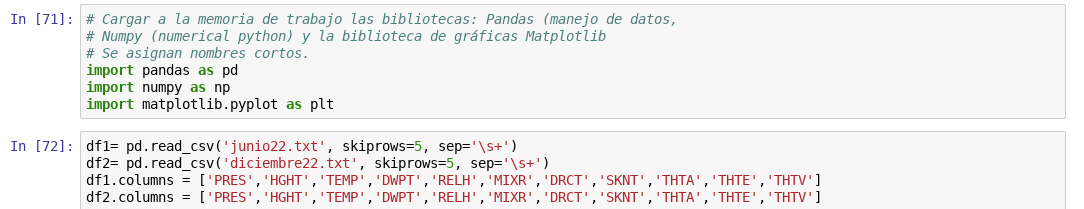
\includegraphics[width=11cm, height=3cm]{def.png}
  \caption{Inicio}
  \label{fig: rap. de vientos y ráfagas}
\end{figure}

\newpage

A continuación se hizo un análisis de los datos, para ver si correspondía lo leído con el archivo original.

\begin{figure}[h!]
  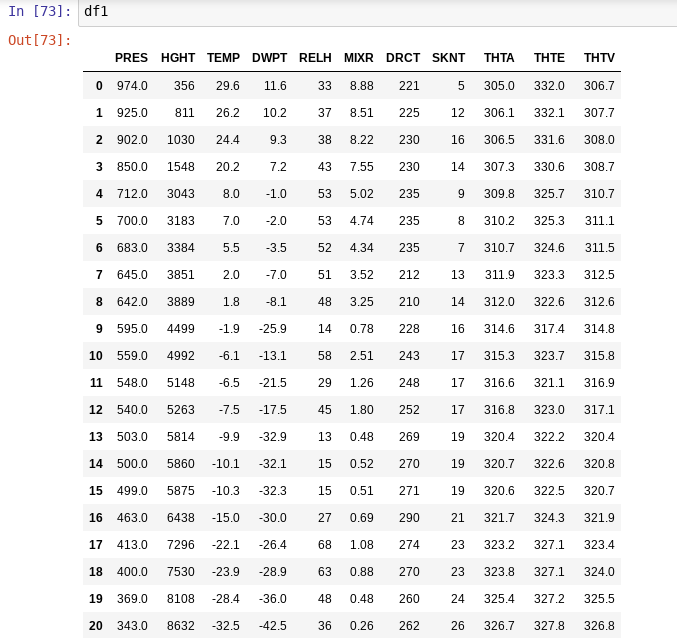
\includegraphics[width=11cm, height=11cm]{datos1.png}
  \caption{Desplegue de los datos del archivo junio}
  \label{fig: rap. de vientos y ráfagas}
\end{figure}

\newpage

\begin{figure}[h!]
  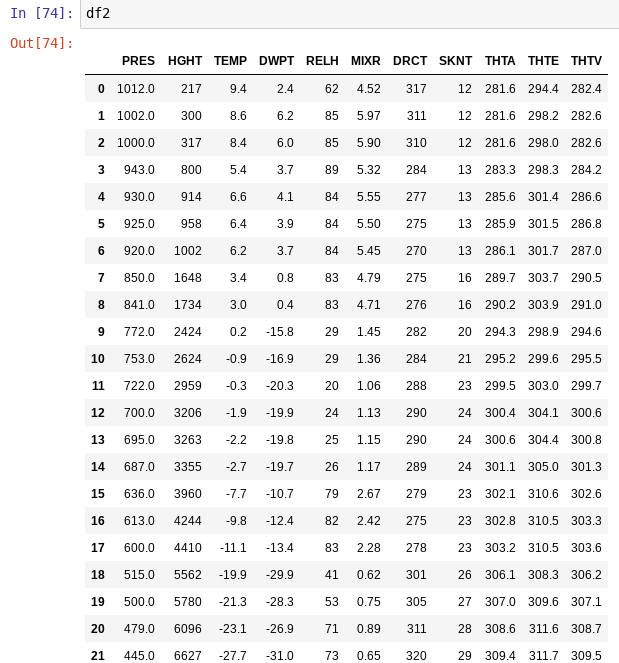
\includegraphics[width=11cm, height=11cm]{datos2.png}
  \caption{Desplegue de los datos de diciembre}
  \label{fig: rap. de vientos y ráfagas}
\end{figure}

lo siguiente fue que se eliminaron líneas innecesarias del archivo de texto que no estaban completas.
Se hizo un análisis del tipo de archivo que contenía cada columna. Algunos archivos no tenían la atribuación de número, sino la de objeto por que se prosiguió a cambiarlo.

\newpage

\begin{figure}[h!]
  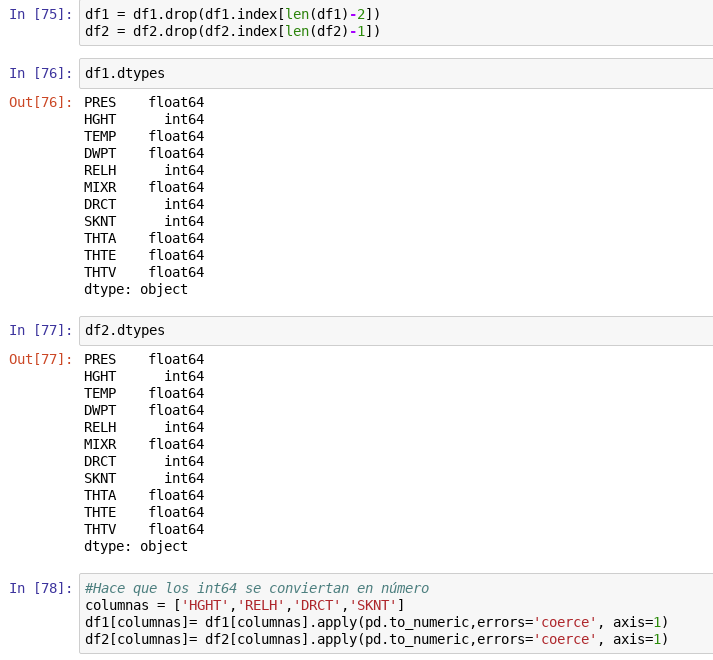
\includegraphics[width=11cm, height=11cm]{objyconv.png}
  \caption{Desplegue de los tipos de datos y su correspondiente conversión a números}
  \label{fig: rap. de vientos y ráfagas}
\end{figure}

A continuación se utilizó la graficación de datos para poder ver de una manera más general el comportamiento de los fenómenos.


\section{Resultados}

Como primer ejercicio, se pide realizar una gráfica para ver la variación de la presióncon respecto a la altura en un lugar para dos distintos meses del año, dando el siguiente resultado

\newpage

\begin{figure}[h!]
\begin{subfigure}{.30\textwidth}
  \
  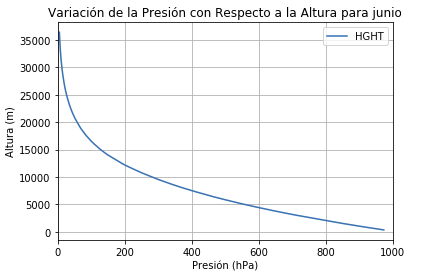
\includegraphics[width=.8\linewidth]{presion1.png}
  \caption{Variación de junio}
  \label{fig:sfig1}
\end{subfigure}
\begin{subfigure}{.30\textwidth}
  \left
  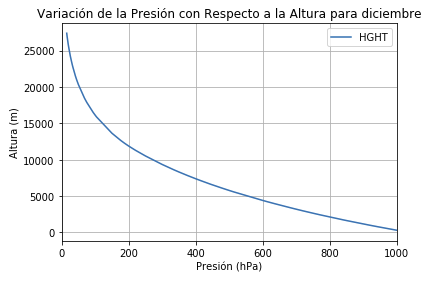
\includegraphics[width=.8\linewidth]{presion2.png}
  \caption{Variación de diciembre}
  \label{fig:sfig2}
\end{subfigure}
\end{figure}

Lo próximo que se hizo fue una gráfica de la tempperatura respecto a la altura, donde se puede apreciar que más allá de los 10 Km no hay presión y tiene un comportamiento lineal registrada para el mes de junio. Mientras para diciembre hay datos un poco más allá de los 25 Km y tiene un comportamiento un poco más errático. Más arriba de la tropopausa no hay mucha presión.

\newpage

\begin{figure}[h!]
\begin{subfigure}{.30\textwidth}
  \
  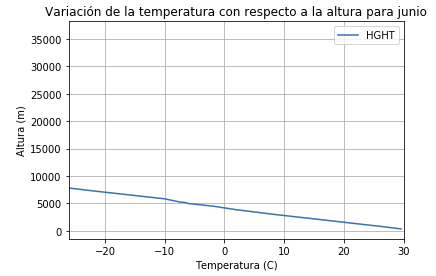
\includegraphics[width=.8\linewidth]{temp1.png}
  \caption{Variación de junio}
  \label{fig:sfig1}
\end{subfigure}
\begin{subfigure}{.30\textwidth}
  \left
  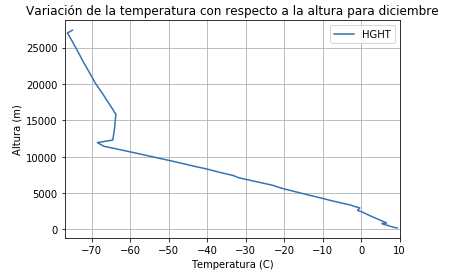
\includegraphics[width=.8\linewidth]{temp2.png}
  \caption{Variación de diciembre}
  \label{fig:sfig2}
\end{subfigure}
\end{figure}

Como tercera parte, se realizó una gráfica donde se veía en una misma, la variación de la temperatura y la temperatura de rocío; donde se aprecia un comportamiento muy similar.

\newpage

\begin{figure}[h!]
\begin{subfigure}{.30\textwidth}
  \
  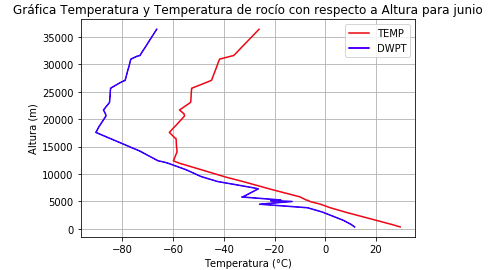
\includegraphics[width=.8\linewidth]{tempr.png}
  \caption{Variación de junio}
  \label{fig:sfig1}
\end{subfigure}
\begin{subfigure}{.30\textwidth}
  \left
  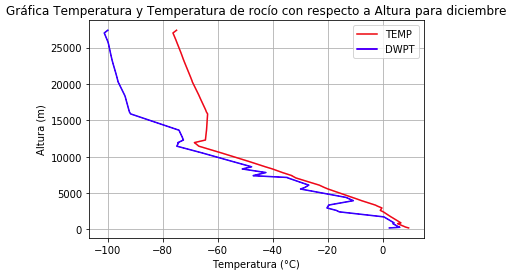
\includegraphics[width=.8\linewidth]{tempr2.png}
  \caption{Variación de diciembre}
  \label{fig:sfig2}
\end{subfigure}
\end{figure}

Lo siguiente fue graficar la rapidez de los vientos en nudos, en el cual se puede observar que a mayor altura crece la cantidad en diciembre, mientras que para junio no parece influir mucho la altura a la que se encuentra.

\newpage

\begin{figure}[h!]
\begin{subfigure}{.30\textwidth}
  \
  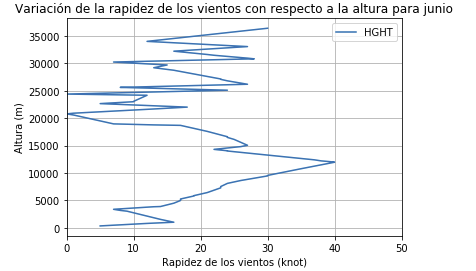
\includegraphics[width=.8\linewidth]{rap.png}
  \caption{Variación de junio}
  \label{fig:sfig1}
\end{subfigure}
\begin{subfigure}{.30\textwidth}
  \left
  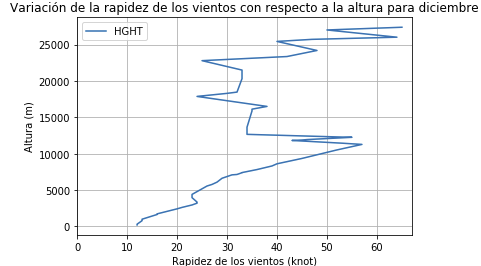
\includegraphics[width=.8\linewidth]{rap2.png}
  \caption{Variación de diciembre}
  \label{fig:sfig2}
\end{subfigure}
\end{figure}

Para finalizar, se obtuvo la graficación de el porcentaje de humedad relativa, cómo influía la altura en éste. Es muy variante respecto a la altura, pero apartir de los diez mil, empieza a decrecer drásticamente

\newpage

\begin{figure}[h!]
\begin{subfigure}{.30\textwidth}
  \
  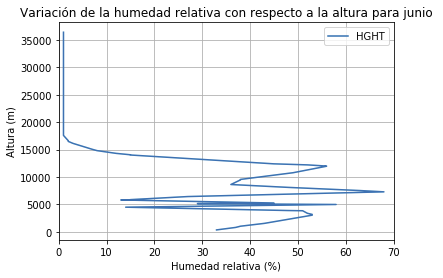
\includegraphics[width=.8\linewidth]{humr.png}
  \caption{Variación de junio}
  \label{fig:sfig1}
\end{subfigure}
\begin{subfigure}{.30\textwidth}
  \left
  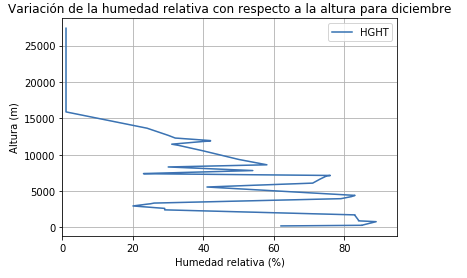
\includegraphics[width=.8\linewidth]{humr2.png}
  \caption{Variación de diciembre}
  \label{fig:sfig2}
\end{subfigure}
\end{figure}

\section{Conclusión}

El graficar en python es muy fácil e intuitivo, cualquier gráfica se puede realizar colocando las correspondientes instrucciones en unas pocas líneas. La actividad fue útil para conocer cómo influye la altura en la propagación de los fenómenos que ocurren en las distintas capas de la atmósfera terrestre. 

\section{Bibliografía}

http://volcano.oregonstate.edu/earths-layers-lesson-1

\\
\\

https://es.sharelatex.com/learn/Inserting_Images

\section{Apéndice}

\itemize

\item¿Cuál es tu opinión general de esta actividad?
\\
Fue una actividad muy intuitiva y tardada que me ayudó a entender a cómo graficar de manera eficiente.

\item¿Qué fue lo que más te agradó? ¿Lo que menos te agradó?
\\
El aprender a graficar bien fue lo más agrdable, lo menos con lo que simpaticé fue la cantidad de errores que no podía percibir, que después corregí.

\item¿Que consideras que aprendiste en esta actividad?
\\
A cómo graficar de manera eficiente y detectar errores en la sintáxis del código. 

\item¿Qué le faltó? ¿O le sobró?
\\
No creo que le haya faltado nada. Se vio cada aspecto de graficación

\item¿Que mejoras sugieres a la actividad?
\\
Que sean menos gráficas, pero de tipo más variado; con diferentes condiciones a cumplir

\enditemize

\end{document}
